\def\retinaface{
    RetinaFace \cite{deng2020retinaface} là một mô hình single-stage giải quyết bài toán Face Detection.
    RetinaFace có kiến trúc mô hình \ref{fig:retinaface_architecture} khá giống với RetinaNet (đã được nêu trong phần)
    TODO: ref phần RetinaNet

    \begin{figure}[H]
        \centering
        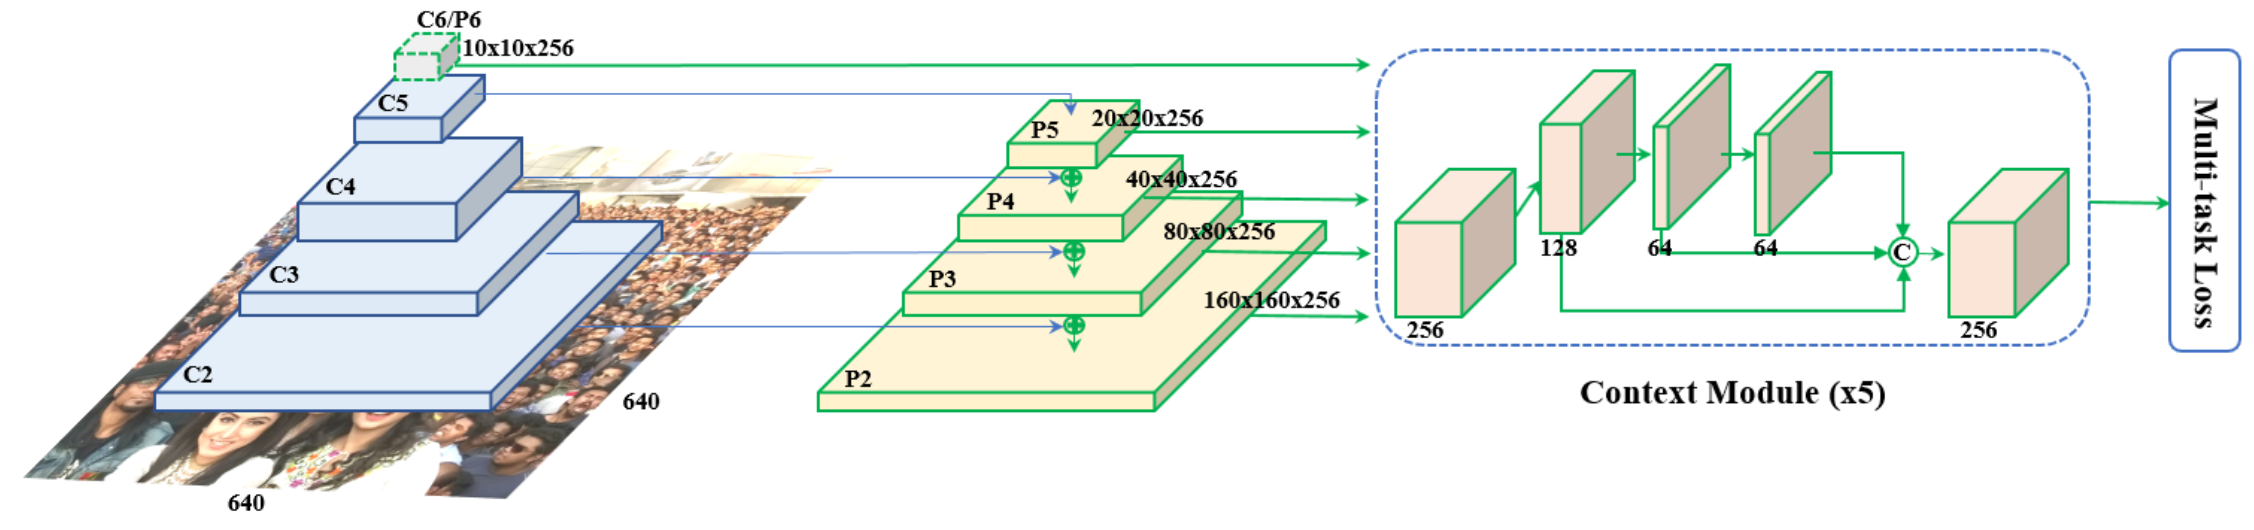
\includegraphics[width=10cm] {images/retinaface_architecture.png}
        \caption{Kiến trúc của mô hình RetinaFace}
        \label{fig:retinaface_architecture}
    \end{figure}

    Nhóm tác giả của RetinaFace đã mang đến bộ dữ liệu và một số kỹ thuật mới giúp cải thiện hiệu năng giải quyết bài toán Face Detection như bộ dữ liệu WIDER FACE với landmarks, 
    TODO: Bổ sung tên các techniques của RetinaFace
    


    \subsubsection{Hàm loss multi-task}
    Trong quá trình train mô hình, với mỗi anchor, RetinaFace tối ưu hàm loss multi-task dưới đây:
    \begin{equation}
        \begin{split}
        L  & =  L_{cls}(p_i, p^{*}_i) + \lambda_1 p^{*}_i L_{box}(t_i, t^{*}_i) + \lambda_2 p^{*}_i L_{pts} (l_i, l^{*}_i) + \lambda_3 p^{*}_i L_{pixel}.\\
        \end{split}
        \label{eq:loss}
    \end{equation}
    Hàm loss trên được gọi là multi-task loss bởi vì nó cùng lúc tối ưu mô hình RetinaFace theo nhiều bài toán con.
    Ta có bốn số hạng của hàm loss tổng, tương ứng với đó là bốn bài toán con mà mô hình sẽ tối ưu: \\
    Phần 1 là hàm loss phân lớp mặt (cụ thể hơn là hàm loss softmax phân lớp nhị phân \textit{là mặt / không là mặt}):
    $L_{cls}(p_i, p^{*}_i)$ với $p_i$ là xác suất mà mô hình dự đoán một anchor có phải là mặt hay không.
    Ta có $p^{*}_i = 1$ nếu anchor đó là mặt còn $p^{*}_i = 0$ nếu anchor đó không phải là mặt. \\
    Phần 2 là hàm loss hồi quy định vị vị trí của bbox:
    $L_{box}(t_i, t^{*}_i)$ với $t_i=\{t_x, t_y, t_w, t_h\}_i$ và $t^{*}_i=\{t^{*}_x, t^{*}_y, t^{*}_w, t^{*}_h\}_i$ lần lượt là bộ bốn tham số đại diện cho toạ độ của anchor mà mô hình dự đoán là mặt và bbox ground-truth từ bộ dữ liệu.
    (toạ độ x của điểm góc trái trên, toạ độ y của điểm góc trái trên, chiều rộng của bbox và chiều cao của bbox)
    We follow~\cite{girshick2015fast} to normalise the box regression targets (centre location, width and height) and use $L_{box}(t_i, t^{*}_i)=R(t_i - t^{*}_i)$, where $R$ is the robust loss function (smooth-L$_1$) defined in~\cite{girshick2015fast}. 
    Phần 3 là hàm loss hồi quy định vị vị trí của landmarks:
    $L_{pts} (l_i, l^{*}_i)$ với $l_i=\{l_{x_1}, l_{y_1}, \dots , l_{x_5}, l_{y_5}\}_i$ và $l^{*}_i=\{l^{*}_{x_1}, l^{*}_{y_1}, \dots , l^{*}_{x_5}, l^{*}_{y_5}\}_i$ represent the predicted five facial landmarks and ground-truth associated with the positive anchor. 
    Similar to the box centre regression, the five facial landmark regression also employs the target normalisation based on the anchor centre.
    (4) Dense regression loss $L_{pixel}$ (refer to Eq.~\ref{fig:selfsupervision}).  
    The loss-balancing parameters $\lambda_1$-$\lambda_3$ are set to 0.25, 0.1 and 0.01, which means that we increase the significance of better box and landmark locations from supervision signals.

    \subsubsection{Kết quả của mô hình RetinaFace}
    \textbf{\textit{Đ}}

    \begin{figure*}[t]
        \centering
        \subfigure[Tập dữ liệu val Dễ]{
        \label{fig:ve}
        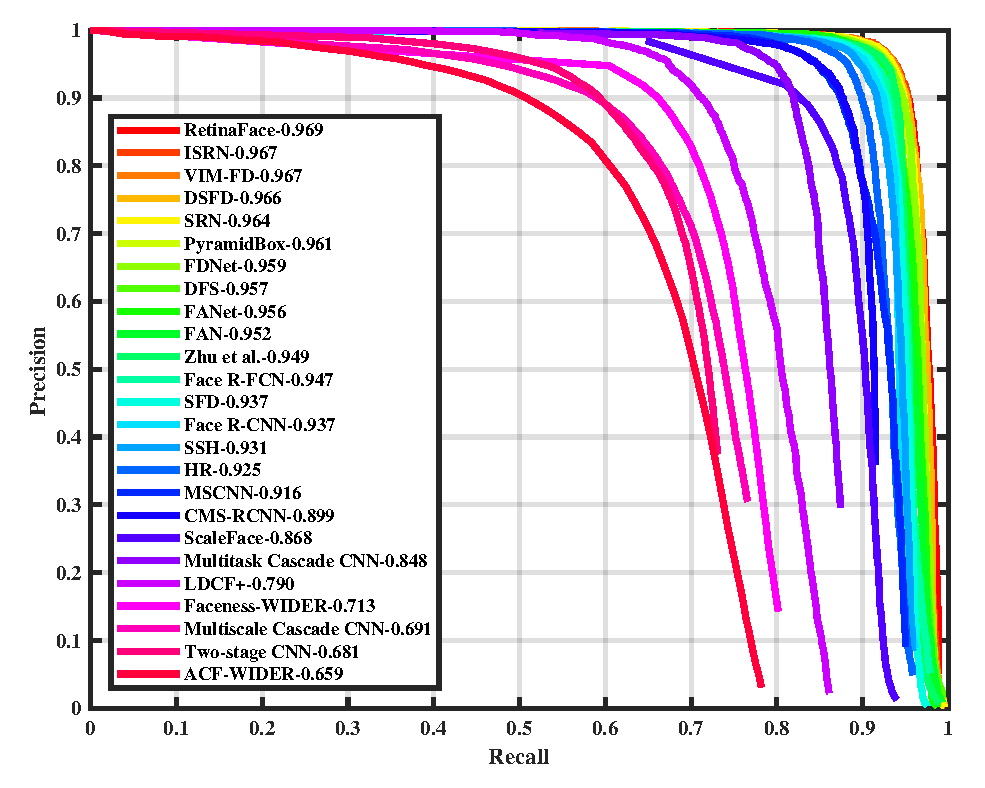
\includegraphics[width=0.32\linewidth]{images/vale.pdf}}
        \subfigure[Tập dữ liệu val Trung bình]{
        \label{fig:vm}
        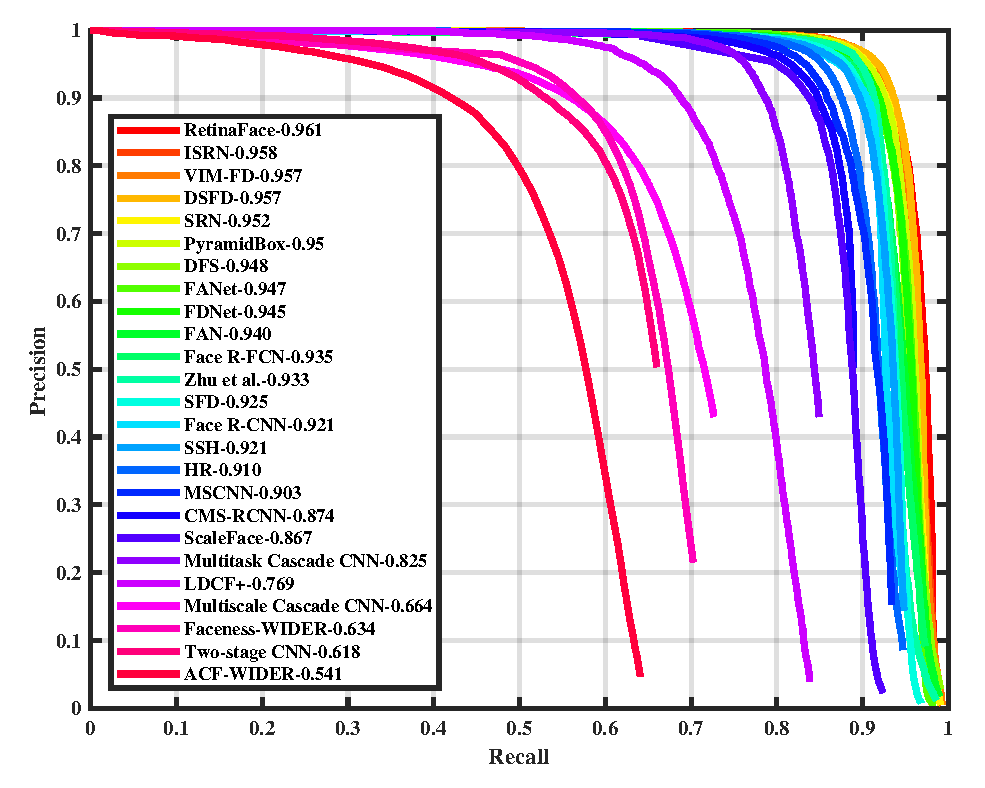
\includegraphics[width=0.32\linewidth]{images/valm.pdf}}
        \subfigure[Tập dữ liệu val Khó]{
        \label{fig:vh}
        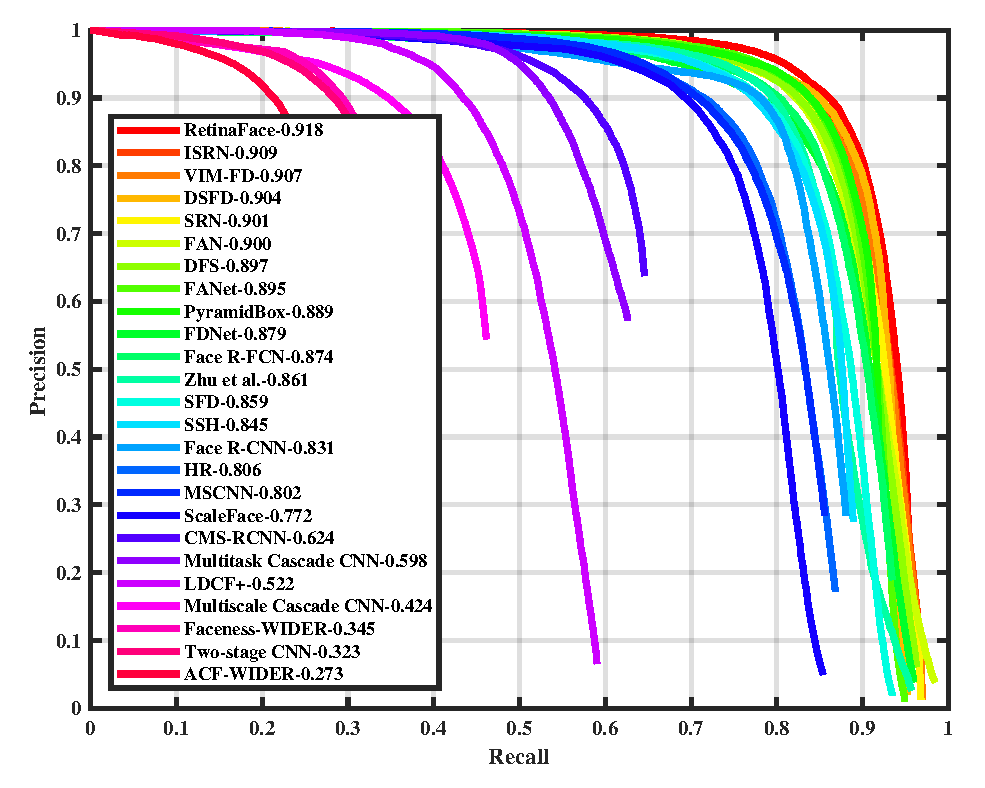
\includegraphics[width=0.32\linewidth]{images/valh.pdf}}
        \subfigure[Tập dữ liệu test Dễ]{
        \label{fig:te}
        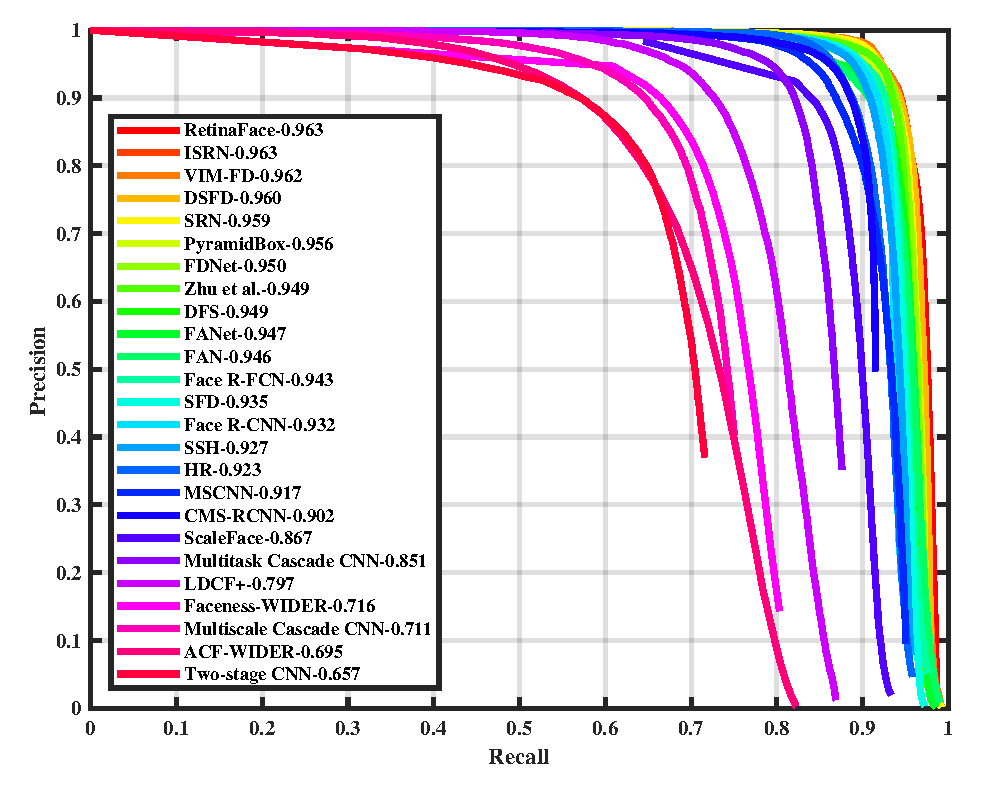
\includegraphics[width=0.32\linewidth]{images/te.pdf}}
        \subfigure[Tập dữ liệu test Trung bình]{
        \label{fig:tm}
        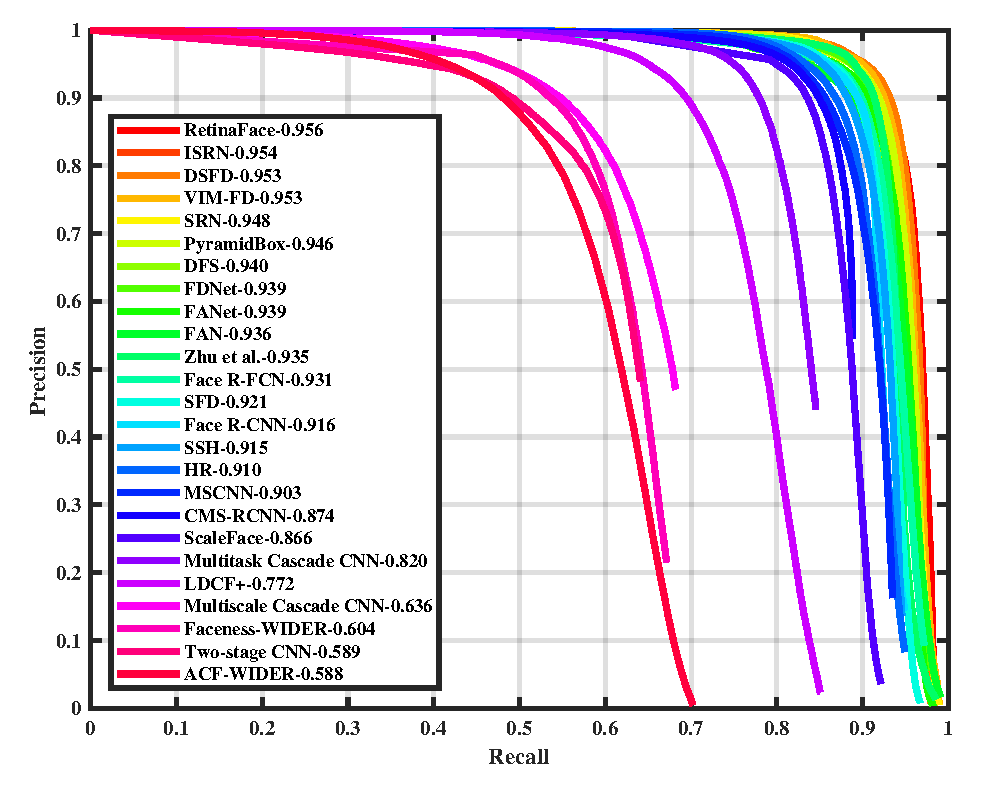
\includegraphics[width=0.32\linewidth]{images/tm.pdf}}
        \subfigure[Tập dữ liệu test Khó]{
        \label{fig:th}
        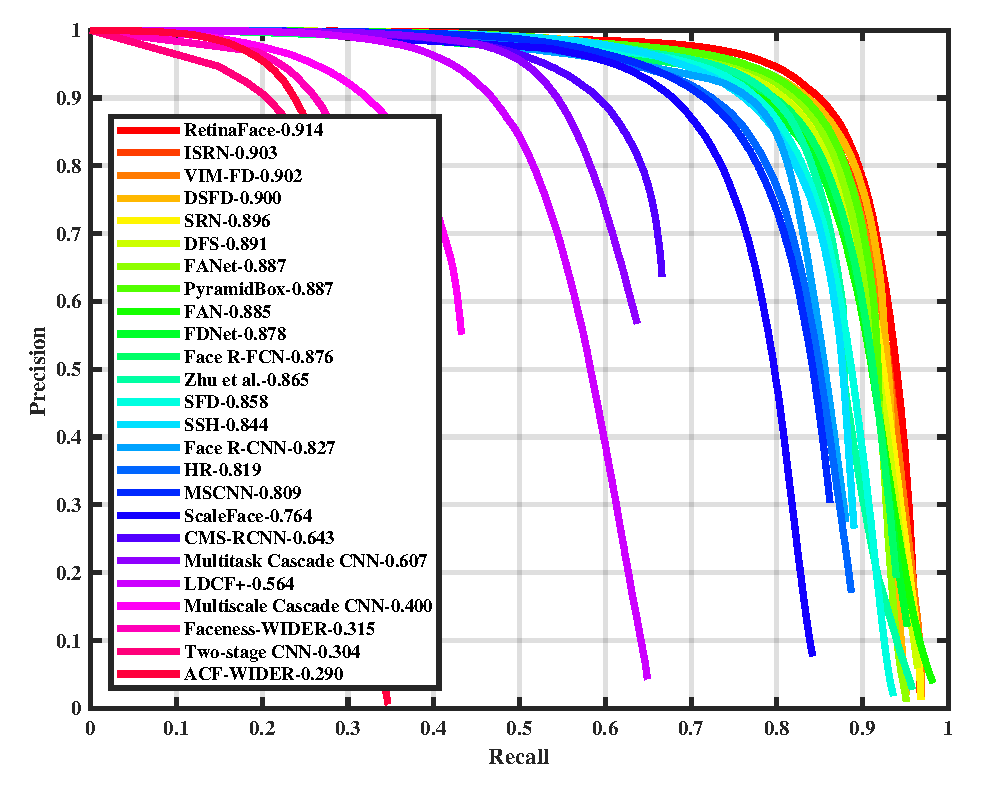
\includegraphics[width=0.32\linewidth]{images/th.pdf}}
        \caption{Đường precision-recall của mô hình RetinaFace trên hai tập dữ liệu val và test của bộ dữ liệu WIDER FACE.}
        \label{fig:wider-face}
    \end{figure*}
}